% ---------------------------------------------------------------- 7 Stack & preprocessing
\begin{frame}{F-SAR stack and preprocessing}
  \begin{columns}[c]
    \begin{column}{0.42\textwidth}
      \small
      \begin{itemize}
        \item Airborne F-SAR stack over an urban test site; primary PS02, secondaries
              selected at training time (PS04/06/08/26) --- the \textbf{reduced stack}.
        \item Per-track acquisition geometry extracted from campaign metadata: per-pixel
              baselines, look angles, slant ranges (consumed by the physics losses, Act VI).
        \item Every artifact is written self-describing: config, stats and geometry ride
              with the data.
      \end{itemize}
    \end{column}
    \begin{column}{0.56\textwidth}
      \centering
      \begin{tikzpicture}
        \draw[soft,thin] (0,5.55) -- (1.9,5.55);
        \fill[accent] (1.45,5.58) circle (0.05);
        \foreach \x/\y in {0.15/6.95, 0.36/6.8, 0.78/6.5, 0.99/6.35} { \draw[soft!50,very thin] (\x,\y) -- (1.45,5.62); \fill[soft] (\x,\y) circle (0.045); }
        \draw[soft!50,very thin] (0.57,6.65) -- (1.45,5.62);
        \fill[accent] (0.57,6.65) circle (0.055);
        \node[font=\scriptsize,text=soft,anchor=east] at (0.42,6.55) {$b_\perp$};
        \node[font=\scriptsize,anchor=north] at (0.95,5.38) {raw F-SAR passes};
        \draw[flow] (2.0,6.05) -- (3.0,6.05);
        \node[font=\scriptsize,text=soft,anchor=south] at (2.5,6.15) {focusing};
        \draw[soft,thin,fill=black!2] (3.42,5.64) rectangle ++(1.1,1.1);
        \draw[soft,thin,fill=black!2] (3.34,5.76) rectangle ++(1.1,1.1);
        \draw[soft,thin,fill=black!2] (3.27,5.55) rectangle ++(1.1,1.1);
        \draw[soft,thin,fill=white] (3.2,5.5) rectangle ++(1.1,1.1);
        \draw[black!8,step=0.22,shift={(3.2,5.5)}] (0,0) grid (1.1,1.1);
        \node[font=\scriptsize,anchor=north] at (3.85,5.35) {focused SLCs (per pass)};
        \draw[flow,rounded corners=3pt] (4.65,6.05) -- (5.3,6.05) -- (5.3,3.5) -- (4.7,3.5);
        \node[font=\scriptsize,text=soft,align=center,anchor=west] at (5.45,4.9) {PyRat\\co-registration};
        \foreach \i in {3,2,1} \draw[soft,thin,fill=black!2] (3.2+0.08*\i,2.95+0.08*\i) rectangle ++(1.1,1.1);
        \draw[soft,thin,fill=white] (3.2,2.95) rectangle ++(1.1,1.1);
        \draw[black!8,step=0.22,shift={(3.2,2.95)}] (0,0) grid (1.1,1.1);
        \node[font=\scriptsize,anchor=south] at (3.75,4.42) {co-registered SLC stack};
        \draw[flow] (3.05,3.5) -- (1.95,3.5);
        \node[font=\scriptsize,text=soft,align=center,anchor=north] at (2.45,3.38) {DEM deramp,\\IFG formation};
        \foreach \i in {3,2,1} \draw[soft,thin,fill=black!2] (0.25+0.08*\i,2.95+0.08*\i) rectangle ++(1.1,1.1);
        \draw[soft,thin,fill=white] (0.25,2.95) rectangle ++(1.1,1.1);
        \begin{scope} \clip (0.25,2.95) rectangle ++(1.1,1.1); \foreach \r in {0.5,0.7,...,2.1} \draw[accent!30,thin] (1.65,2.5) circle (\r); \end{scope}
        \node[font=\scriptsize,anchor=south] at (0.9,4.42) {IFG stack};
        \draw[flow] (0.75,2.85) -- (0.75,1.55);
        \node[font=\scriptsize,text=soft,align=center,anchor=west] at (0.95,2.2) {boxcar $20{\times}20$ multilook,\\covariance estimation};
        \draw[soft,thin,fill=white] (0.0,0.1) rectangle ++(1.3,1.3);
        \begin{scope} \clip (0.0,0.1) rectangle ++(1.3,1.3); \foreach \r in {0.65,1.05,...,2.75} \draw[accent!15,thick] (1.35,-0.45) circle (\r); \end{scope}
        \draw[accent,thick] (0.3,0.7) rectangle ++(0.5,0.26);
        \node[font=\scriptsize,anchor=north] at (0.65,-0.05) {covariance stack};
        \draw[flow] (1.45,0.75) -- (3.15,0.75);
        \node[font=\scriptsize,text=soft,align=center,anchor=south] at (2.2,0.9) {Capon\\$z\in[-20,80]$\,m};
        \draw[soft,thin,fill=black!2] (3.3,0.1) rectangle ++(1.6,1.3);
        \draw[->,soft] (3.4,0.2) -- (3.4,1.3);
        \node[font=\scriptsize,text=soft,anchor=west] at (3.44,1.2) {$z$};
        \draw[accent,thick] plot[smooth] coordinates {(3.55,0.42) (3.8,0.38) (4.05,0.47) (4.3,0.4) (4.55,0.45)};
        \draw[accent!55,thick] (3.65,0.95) -- (3.95,0.95);
        \draw[accent!55,thick] (4.2,0.82) -- (4.55,0.82);
        \node[font=\scriptsize,anchor=north] at (4.1,-0.05) {Capon tomogram};
      \end{tikzpicture}
    \end{column}
  \end{columns}
\end{frame}

% ---------------------------------------------------------------- 8a Peak init
\begin{frame}{Before the fit: prominence-ranked initialisation}
  \begin{columns}[T]
    \begin{column}{0.60\textwidth}
      \centering
      \begin{tikzpicture}[scale=1.55]
        \draw[->,soft] (0,0) -- (3.75,0) node[right,font=\scriptsize]{$z$};
        \draw[->,soft] (0,0) -- (0,1.75) node[above,font=\scriptsize]{$p(z)$};
        \draw[soft,thin,domain=0.05:3.55,samples=160,smooth]
          plot (\x,{1.30*exp(-(\x-0.95)^2/(2*0.10)) + 0.70*exp(-(\x-2.25)^2/(2*0.09))
                    + 0.18*exp(-(\x-3.15)^2/(2*0.02)) + 0.06*exp(-(\x-0.35)^2/(2*0.008))
                    + 0.04*exp(-(\x-1.55)^2/(2*0.008)) + 0.04*exp(-(\x-2.70)^2/(2*0.008)) + 0.05});
        \draw[soft,dashed,thin] (1.65,0.28) -- (2.72,0.28);
        \draw[{Stealth[length=1.4mm]}-{Stealth[length=1.4mm]},ink!70,thin] (2.25,0.28) -- (2.25,0.73);
        \node[font=\tiny,text=ink!70,anchor=east] at (2.17,0.50) {prominence};
        \fill[accent] (0.95,1.35) circle (1.0pt);
        \fill[accent] (2.25,0.75) circle (1.0pt);
        \draw[soft]   (3.15,0.24) circle (1.0pt);
        \node[circle,draw=accent,fill=white,inner sep=0.7pt,font=\tiny,text=accent] at (0.95,1.52) {1};
        \node[circle,draw=accent,fill=white,inner sep=0.7pt,font=\tiny,text=accent] at (2.25,0.92) {2};
        \node[circle,draw=soft,fill=white,inner sep=0.7pt,font=\tiny,text=soft] at (3.15,0.40) {3};
        \node[font=\tiny,text=soft] at (3.15,0.57) {dropped ($K{=}2$)};
      \end{tikzpicture}
      \\[2pt]
      {\scriptsize \textcolor{soft}{Raw Capon spectrum}; \textcolor{accent}{peaks ranked by
       prominence, top $K$ kept}.}
    \end{column}
    \begin{column}{0.38\textwidth}
      \centering
      \begin{tikzpicture}[scale=1.15]
        \fill[accent!12]
          plot[domain=0.25:1.548,samples=40,smooth] (\x,{0.7*exp(-(\x-2.0)^2/0.605)})
          -- plot[domain=1.548:2.8,samples=40,smooth] (\x,{1.0*exp(-(\x-0.9)^2/0.605)})
          -- (2.8,0) -- (0.25,0) -- cycle;
        \draw[->,soft] (0,0) -- (3.15,0) node[right,font=\tiny]{$z$};
        \draw[accent,thin,domain=0.05:3.0,samples=60,smooth]
          plot (\x,{1.0*exp(-(\x-0.9)^2/0.605)});
        \draw[accent!60,thin,domain=0.05:3.0,samples=60,smooth]
          plot (\x,{0.7*exp(-(\x-2.0)^2/0.605)});
        \node[font=\tiny,text=soft] at (1.45,0.20) {overlap};
      \end{tikzpicture}
      \\[-1pt]
      {\tiny wide $\sigma$ start: overlapping components, coupled gradients}
      \\[7pt]
      \begin{tikzpicture}[scale=1.15]
        \draw[->,soft] (0,0) -- (3.15,0) node[right,font=\tiny]{$z$};
        \draw[accent,thin,domain=0.05:3.0,samples=60,smooth]
          plot (\x,{1.0*exp(-(\x-0.9)^2/0.097)});
        \draw[accent!60,thin,domain=0.05:3.0,samples=60,smooth]
          plot (\x,{0.7*exp(-(\x-2.0)^2/0.097)});
      \end{tikzpicture}
      \\[-1pt]
      {\tiny small $\sigma_0$ start: disjoint components, easier convergence}
    \end{column}
  \end{columns}
  \vspace{4pt}
  \footnotesize
  \begin{itemize}
    \item Candidate scatterers: local maxima with prominence $\geq 5\%$ of the pixel
          maximum, separated by at least the initial width $\sigma_0$.
    \item Ranked by prominence, top $K$ kept --- $\mu_k$, $a_k$ read directly at the
          surviving peaks; every component starts at the shared width guess
          $\sigma_0 = \max(2\,\Delta\xi,\ \mathrm{span}/8K)$, with $\Delta\xi$ the
          elevation grid step and $\mathrm{span} = \xi_N - \xi_1$ the full grid
          extent ($100$\,m here): an eighth of a component's even share of the
          axis, floored at two grid bins --- deliberately small, so components
          start disjoint and their gradients decouple (right).
    \item Degenerate pixels handled explicitly: fewer than $K$ peaks $\to$ argmax of the
          peak-masked residual; empty profile $\to$ uniform spread over the grid.
  \end{itemize}
\end{frame}

% ---------------------------------------------------------------- 8 Ground truth
\begin{frame}{Ground truth: fitted Gaussian parameters}
  \small
  \begin{columns}[T]
    \begin{column}{0.55\textwidth}
      \begin{minipage}[t][0.68\textheight]{\linewidth}
      \vfill
      Supervised target: the per-pixel array $[a_k,\mu_k,\sigma_k]_{k=1}^{K}$
      ($K{=}2$ today, $K{=}5$ in development), fit to the per-pixel max-normalised
      Capon spectrum $\tilde p = p/p_{\max}$ on the elevation grid $\xi_n$:
      \[
        \mathcal{L} \;=\; \frac{1}{N}\sum_{n=1}^{N}\big(\hat p(\xi_n)-\tilde p(\xi_n)\big)^{2},
        \qquad
        \hat p(\xi) = \sum_{k} a_k\, e^{-\frac{(\xi-\mu_k)^2}{2\sigma_k^2}}
      \]
      \vfill
      One shared loss; each parameter group takes its own projected Adam step:
      \[
        \begin{aligned}
          a_k      &\;\leftarrow\; \big[\, a_k - \eta\,\mathrm{Adam}(\partial_{a_k}\mathcal{L}) \,\big]_{+} \\[-1pt]
          \mu_k    &\;\leftarrow\; \operatorname{clip}_{[\mu^-\!,\;\mu^+]}\big( \mu_k - \eta\,\mathrm{Adam}(\partial_{\mu_k}\mathcal{L}) \big) \\[-1pt]
          \sigma_k &\;\leftarrow\; \operatorname{clip}_{[\sigma^-\!,\;\sigma^+]}\big( \sigma_k - \eta\,\mathrm{Adam}(\partial_{\sigma_k}\mathcal{L}) \big)
        \end{aligned}
      \]
      \vfill
      \end{minipage}
    \end{column}
    \begin{column}{0.43\textwidth}
      \centering
      \begin{tikzpicture}[scale=1.25]
        \draw[->,soft] (0,0) -- (3.75,0) node[right,font=\scriptsize]{$z$};
        \draw[->,soft] (0,0) -- (0,1.75) node[above,font=\scriptsize]{$p(z)$};
        \draw[soft,thin,domain=0.05:3.55,samples=160,smooth]
          plot (\x,{1.30*exp(-(\x-0.95)^2/(2*0.10)) + 0.70*exp(-(\x-2.25)^2/(2*0.09))
                    + 0.18*exp(-(\x-3.15)^2/(2*0.02)) + 0.06*exp(-(\x-0.35)^2/(2*0.008))
                    + 0.04*exp(-(\x-1.55)^2/(2*0.008)) + 0.04*exp(-(\x-2.70)^2/(2*0.008)) + 0.05});
        \draw[accent!55,thin,dashed,domain=0.05:3.55,samples=90,smooth]
          plot (\x,{1.35*exp(-(\x-0.95)^2/(2*0.048)) + 0.75*exp(-(\x-2.25)^2/(2*0.048))});
        \draw[accent,thick,domain=0.05:3.55,samples=90,smooth]
          plot (\x,{1.32*exp(-(\x-0.95)^2/(2*0.115)) + 0.72*exp(-(\x-2.25)^2/(2*0.10))});
        \draw[soft,dashed,thin] (0.95,0) -- (0.95,1.32);
        \draw[soft,dashed,thin] (2.25,0) -- (2.25,0.72);
        \draw[soft,dashed,thin] (0,1.32) -- (0.95,1.32);
        \draw[{Stealth[length=1.4mm]}-{Stealth[length=1.4mm]},accent!75,thin]
          (0.95,0.80) -- (1.29,0.80);
        \node[font=\scriptsize,accent,anchor=north] at (0.95,-0.04) {$\mu_1$};
        \node[font=\scriptsize,accent,anchor=north] at (2.25,-0.04) {$\mu_2$};
        \node[font=\scriptsize,accent,anchor=east]  at (-0.04,1.32) {$a_1$};
        \node[font=\scriptsize,accent,anchor=south] at (1.12,0.82) {$\sigma_1$};
      \end{tikzpicture}
      \\[2pt]
      {\scriptsize Same pixel: \textcolor{soft}{Capon spectrum},
       \textcolor{accent!60}{peak initialisation (dashed)},
       \textcolor{accent}{converged fit}; the fitted $[a_k,\mu_k,\sigma_k]$ are the label.}
      \begin{itemize}
        \item {\footnotesize Fitted in normalised space; the winning amplitudes are
              denormalised back, $a_k \to p_{\max}\, a_k$ ($\mu_k$, $\sigma_k$ already
              live on the physical axis).}
        \item {\footnotesize All pixels batched in one optimisation --- not a per-pixel
              loop (next slide); most pixels activate one or two Gaussians (Act III).}
      \end{itemize}
    \end{column}
  \end{columns}
\end{frame}

% ---------------------------------------------------------------- 8a2 Label distributions
\begin{frame}{What the labels look like: fitted parameter distributions}
  \begin{columns}[T]
    \begin{column}{0.32\textwidth}
      \centering
      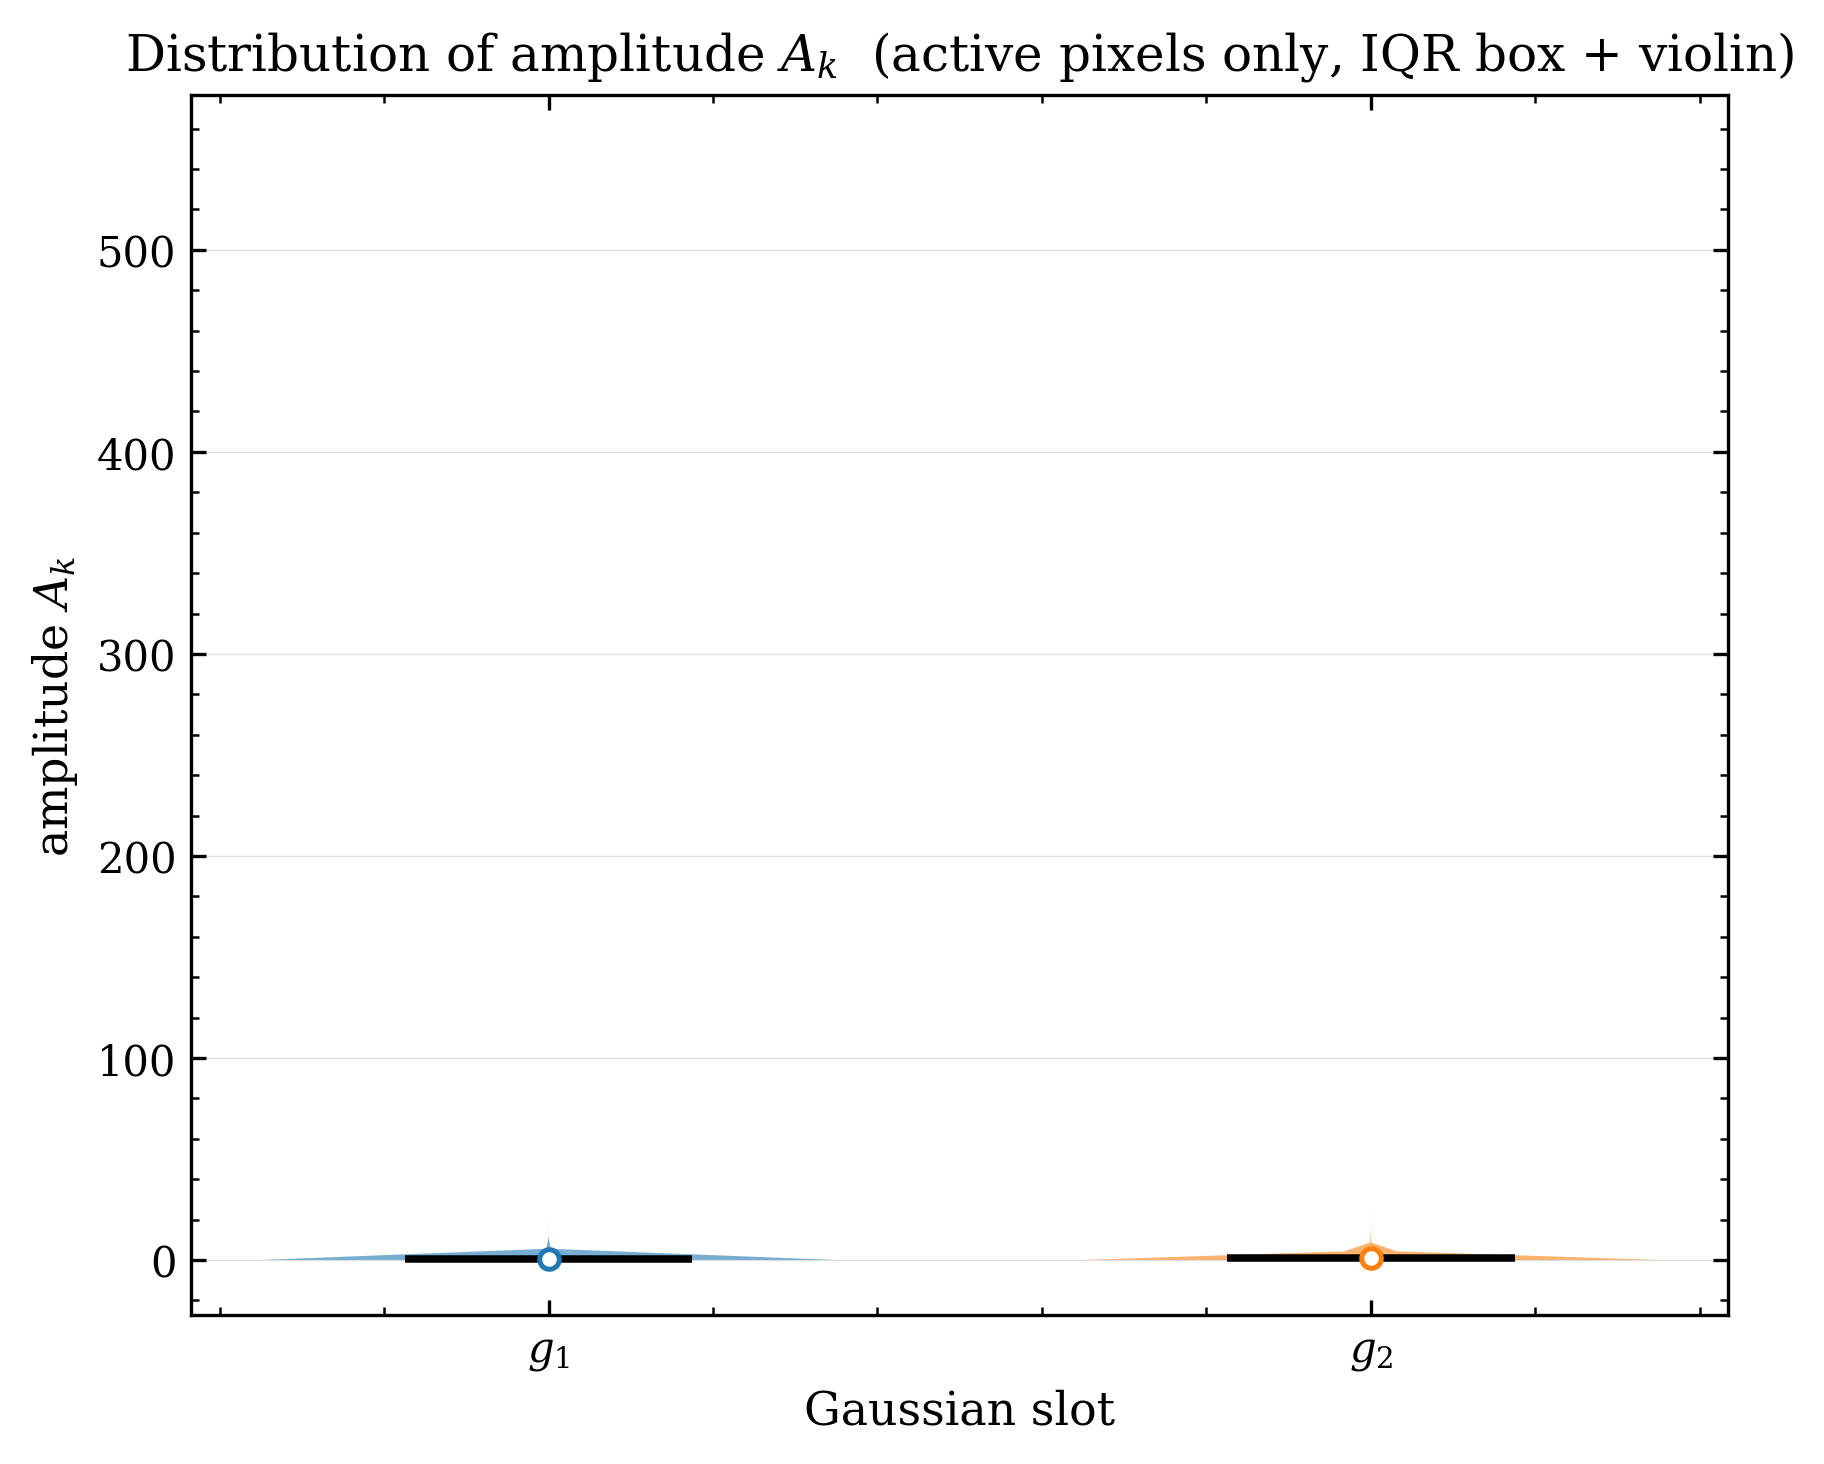
\includegraphics[width=\linewidth]{../figures/param_extraction/label_distributions/amp_distribution.png}
    \end{column}
    \begin{column}{0.32\textwidth}
      \centering
      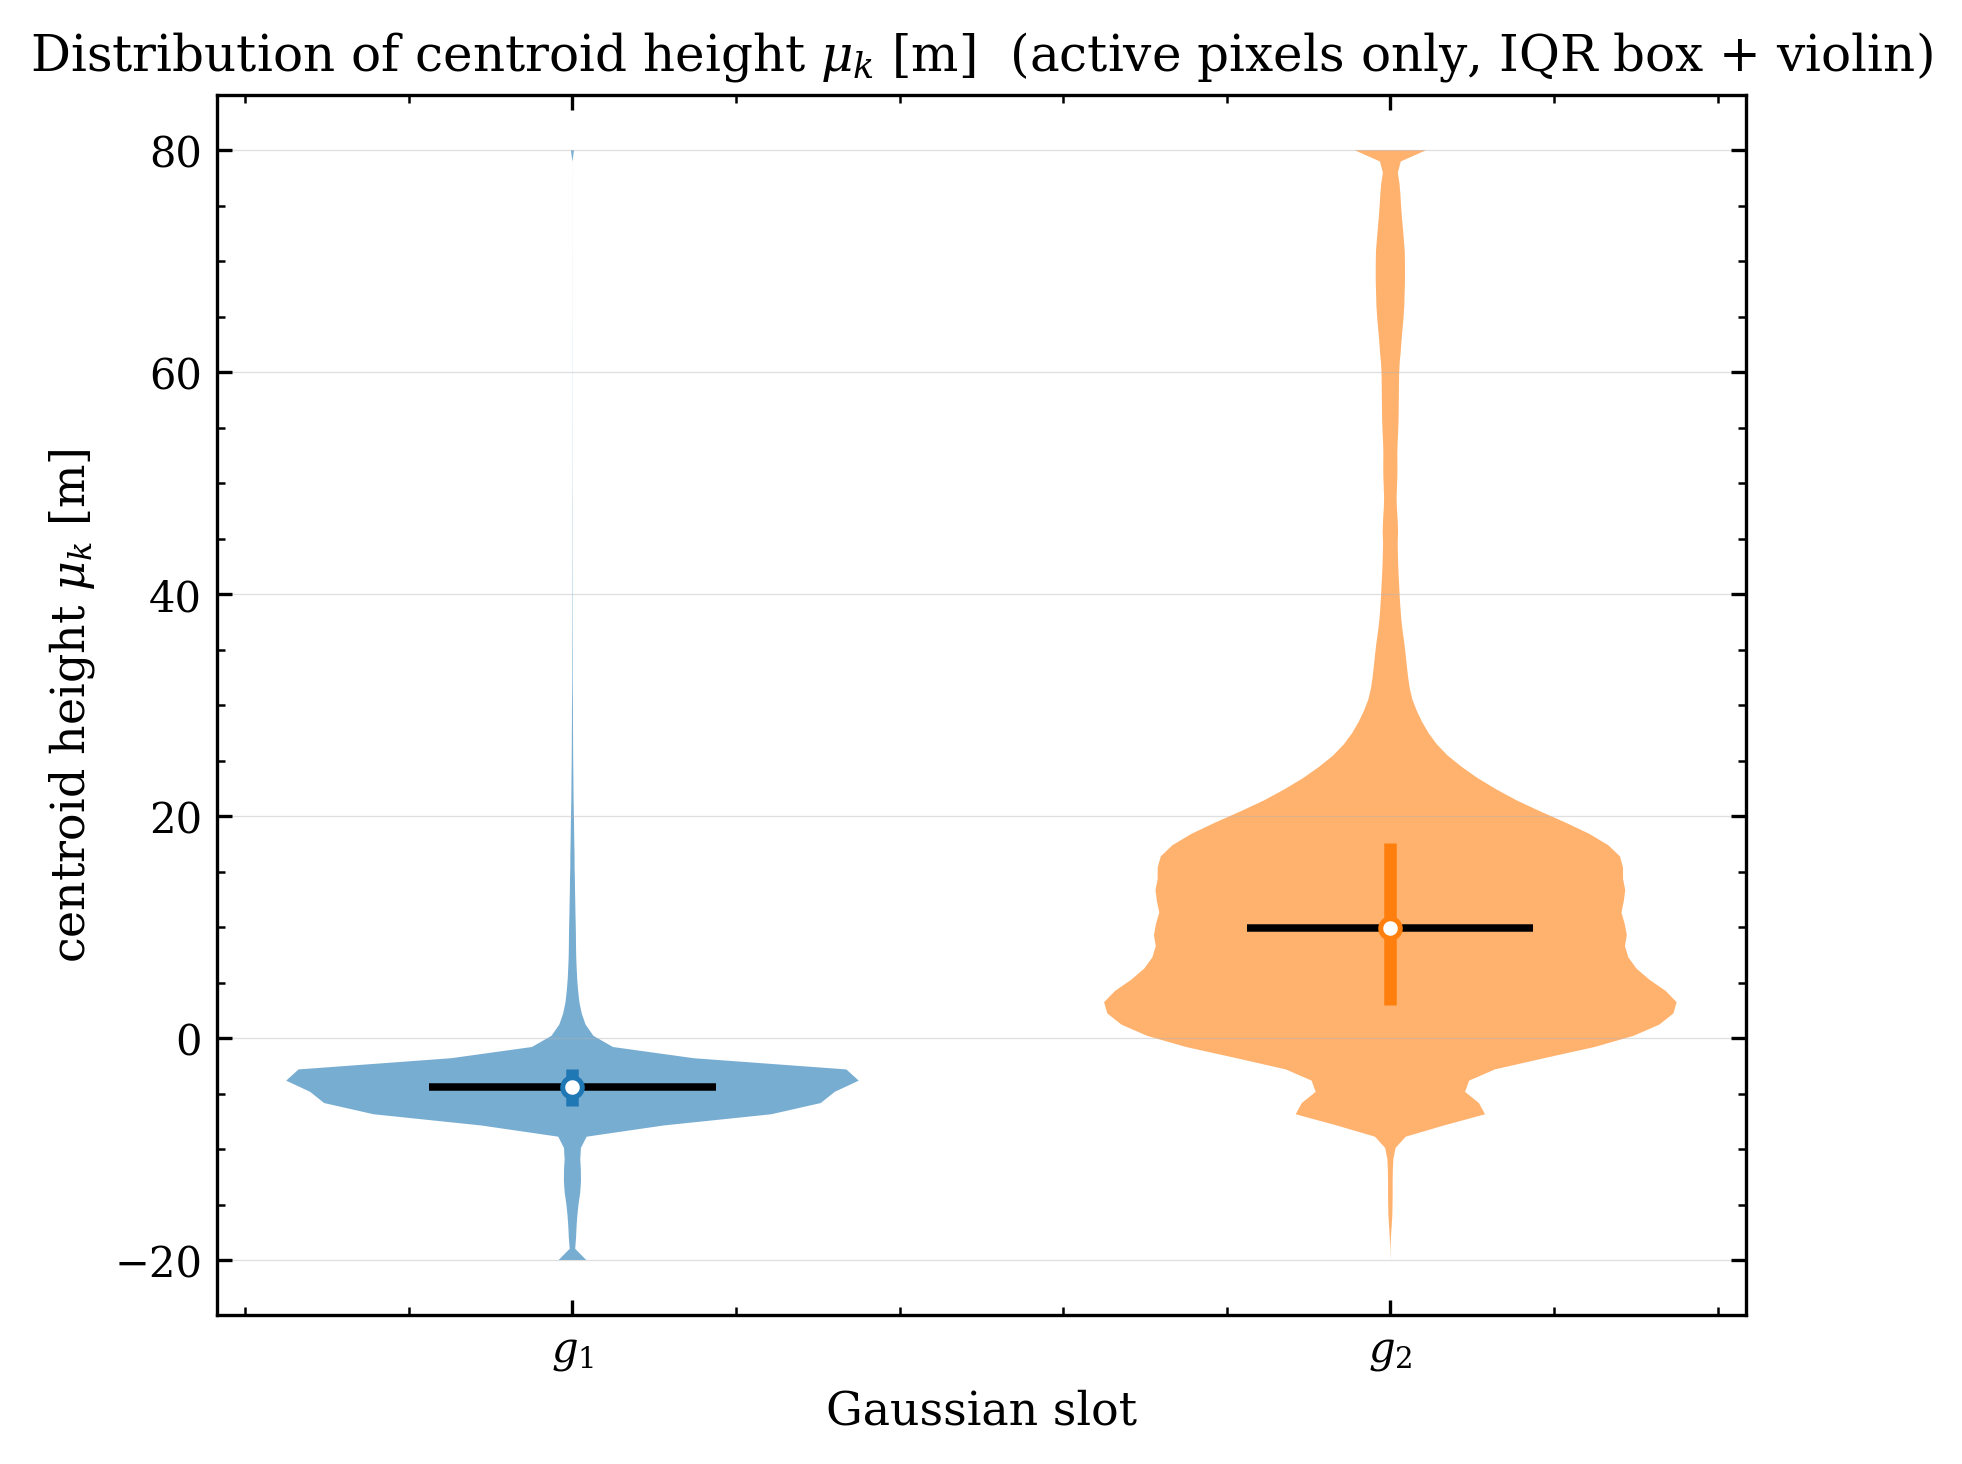
\includegraphics[width=\linewidth]{../figures/param_extraction/label_distributions/mu_distribution.png}
    \end{column}
    \begin{column}{0.32\textwidth}
      \centering
      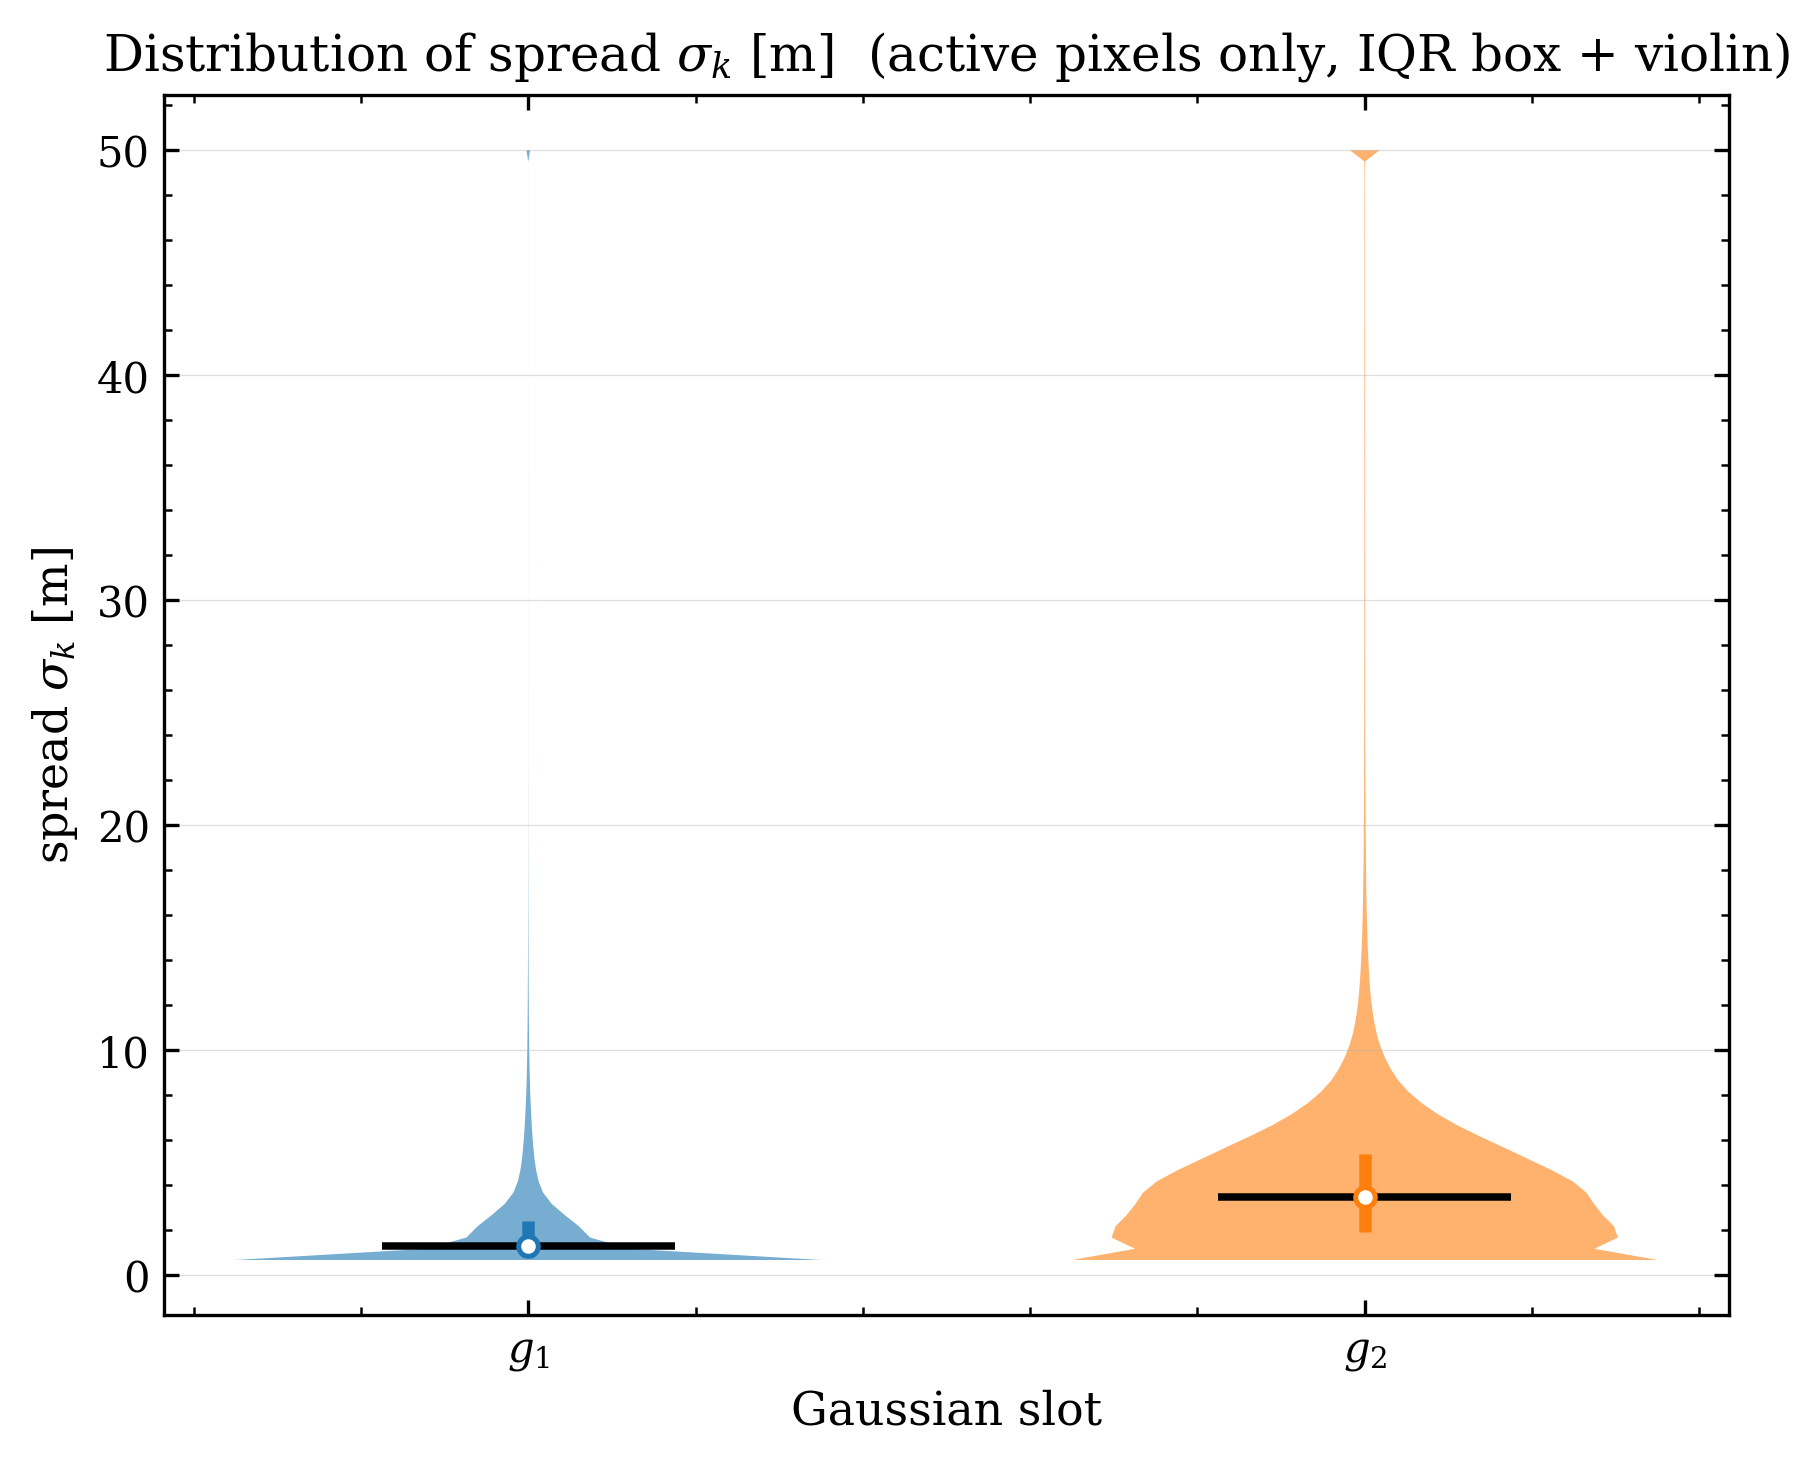
\includegraphics[width=\linewidth]{../figures/param_extraction/label_distributions/sigma_distribution.png}
    \end{column}
  \end{columns}
  \vspace{2pt}
  \small
  \begin{itemize}
    \item Distributions of the supervised targets $[a_k,\mu_k,\sigma_k]$ over \textbf{active pixels only}, split by slot ($g_1$, $g_2$; IQR box $+$ violin).
    \item The second slot $g_2$ sits \textbf{higher} ($\mu_2\!\approx\!10$\,m vs $\mu_1\!\approx\!-5$\,m) and \textbf{broader} ($\sigma_2$ heavier-tailed) --- it takes the elevated, more diffuse scatterer when a pixel activates two.
    \item Amplitudes stay small and tightly peaked; $\mu$ and $\sigma$ carry the long tails the robust scaling (previous act) is built for.
  \end{itemize}
\end{frame}

% ---------------------------------------------------------------- 8b Best-K selection
\begin{frame}{Choosing $K$: fit every order, penalise complexity}
  \begin{columns}[T]
    \begin{column}{0.56\textwidth}
      \footnotesize
      \begin{itemize}
        \item Every active pixel is fitted at \emph{every} order $K = 1,\dots,K_{\max}$,
              all sharing the same peak init (top-$K$ slice).
        \item Per-pixel selection by penalised score
              \[
                S(K) \;=\; \underbrace{\mathrm{MSE}_K}_{\text{fitting component}}
                \;+\; \underbrace{\lambda_K\, K}_{\text{regularization component}}
              \]
              per-$K$ MSE, penalised scores and the best-$K$
              map ride with the dataset as diagnostics.
        \item Today's $K{=}2$ labels run with $\lambda_K = 0$: the fitting component alone
              decides --- the regularization component becomes load-bearing for the $K{=}5$
              extension.
      \end{itemize}
      \vspace{6pt}
      \centering
      \begin{tikzpicture}[xscale=1.45,yscale=1.15]
        \draw[->,soft] (0,0) -- (3.3,0) node[right,font=\tiny]{$K$};
        \draw[->,soft] (0,0) -- (0,1.6) node[above,font=\tiny]{score};
        \foreach \k in {1,...,5} {
          \draw[soft] (0.55*\k,0) -- (0.55*\k,-0.04);
          \node[font=\tiny,text=soft,anchor=north] at (0.55*\k,-0.05) {\k};
        }
        \draw[soft,thin] (0.55,1.31) -- (1.10,0.38) -- (1.65,0.30) -- (2.20,0.27) -- (2.75,0.25);
        \foreach \p in {(0.55,1.31),(1.10,0.38),(1.65,0.30),(2.20,0.27),(2.75,0.25)}
          \fill[soft] \p circle (0.8pt);
        \draw[accent,thick] (0.55,1.42) -- (1.10,0.60) -- (1.65,0.63) -- (2.20,0.71) -- (2.75,0.80);
        \foreach \p in {(0.55,1.42),(1.10,0.60),(1.65,0.63),(2.20,0.71),(2.75,0.80)}
          \fill[accent] \p circle (0.8pt);
        \draw[good,thick] (1.10,0.60) circle (2.4pt);
        \node[font=\tiny,text=good,anchor=south] at (1.80,1.18) {best $K$};
        \draw[good,thin] (1.74,1.16) -- (1.19,0.69);
        \node[font=\tiny,text=soft,anchor=west] at (2.85,0.20) {$\mathrm{MSE}_K$};
        \node[font=\tiny,text=accent,anchor=south west] at (2.28,0.86) {$\mathrm{MSE}_K + \lambda_K K$};
      \end{tikzpicture}
    \end{column}
    \begin{column}{0.42\textwidth}
      \centering
      \begin{tikzpicture}[xscale=1.45,yscale=1.02]
        \draw[->,soft] (0,0) -- (3.75,0);
        \draw[soft,thin,domain=0.05:3.55,samples=140,smooth]
          plot (\x,{1.30*exp(-(\x-0.95)^2/(2*0.10)) + 0.70*exp(-(\x-2.25)^2/(2*0.09))
                    + 0.18*exp(-(\x-3.15)^2/(2*0.02)) + 0.06*exp(-(\x-0.35)^2/(2*0.008))
                    + 0.04*exp(-(\x-1.55)^2/(2*0.008)) + 0.04*exp(-(\x-2.70)^2/(2*0.008)) + 0.05});
        \draw[accent,thick,domain=0.05:3.55,samples=80,smooth]
          plot (\x,{1.28*exp(-(\x-0.98)^2/(2*0.13))});
      \end{tikzpicture}
      \\[-1pt]
      {\tiny $K{=}1$: second scatterer missed}
      \\[6pt]
      \begin{tikzpicture}[xscale=1.45,yscale=1.02]
        \draw[->,soft] (0,0) -- (3.75,0);
        \draw[soft,thin,domain=0.05:3.55,samples=140,smooth]
          plot (\x,{1.30*exp(-(\x-0.95)^2/(2*0.10)) + 0.70*exp(-(\x-2.25)^2/(2*0.09))
                    + 0.18*exp(-(\x-3.15)^2/(2*0.02)) + 0.06*exp(-(\x-0.35)^2/(2*0.008))
                    + 0.04*exp(-(\x-1.55)^2/(2*0.008)) + 0.04*exp(-(\x-2.70)^2/(2*0.008)) + 0.05});
        \draw[accent,thick,domain=0.05:3.55,samples=80,smooth]
          plot (\x,{1.32*exp(-(\x-0.95)^2/(2*0.115)) + 0.72*exp(-(\x-2.25)^2/(2*0.10))});
      \end{tikzpicture}
      \\[-1pt]
      {\tiny $K{=}2$: both scatterers captured}
      \\[6pt]
      \begin{tikzpicture}[xscale=1.45,yscale=1.02]
        \draw[->,soft] (0,0) -- (3.75,0);
        \draw[soft,thin,domain=0.05:3.55,samples=140,smooth]
          plot (\x,{1.30*exp(-(\x-0.95)^2/(2*0.10)) + 0.70*exp(-(\x-2.25)^2/(2*0.09))
                    + 0.18*exp(-(\x-3.15)^2/(2*0.02)) + 0.06*exp(-(\x-0.35)^2/(2*0.008))
                    + 0.04*exp(-(\x-1.55)^2/(2*0.008)) + 0.04*exp(-(\x-2.70)^2/(2*0.008)) + 0.05});
        \draw[accent,thick,domain=0.05:3.55,samples=80,smooth]
          plot (\x,{1.32*exp(-(\x-0.95)^2/(2*0.115)) + 0.72*exp(-(\x-2.25)^2/(2*0.10))
                    + 0.17*exp(-(\x-3.15)^2/(2*0.03))});
      \end{tikzpicture}
      \\[-1pt]
      {\tiny $K{=}3$: marginal MSE gain}
    \end{column}
  \end{columns}
\end{frame}

% ---------------------------------------------------------------- 8c Best-K map
\begin{frame}{The best-$K$ map: where the second scatterer lives}
  \begin{columns}[c]
    \begin{column}{0.62\textwidth}
      \centering
      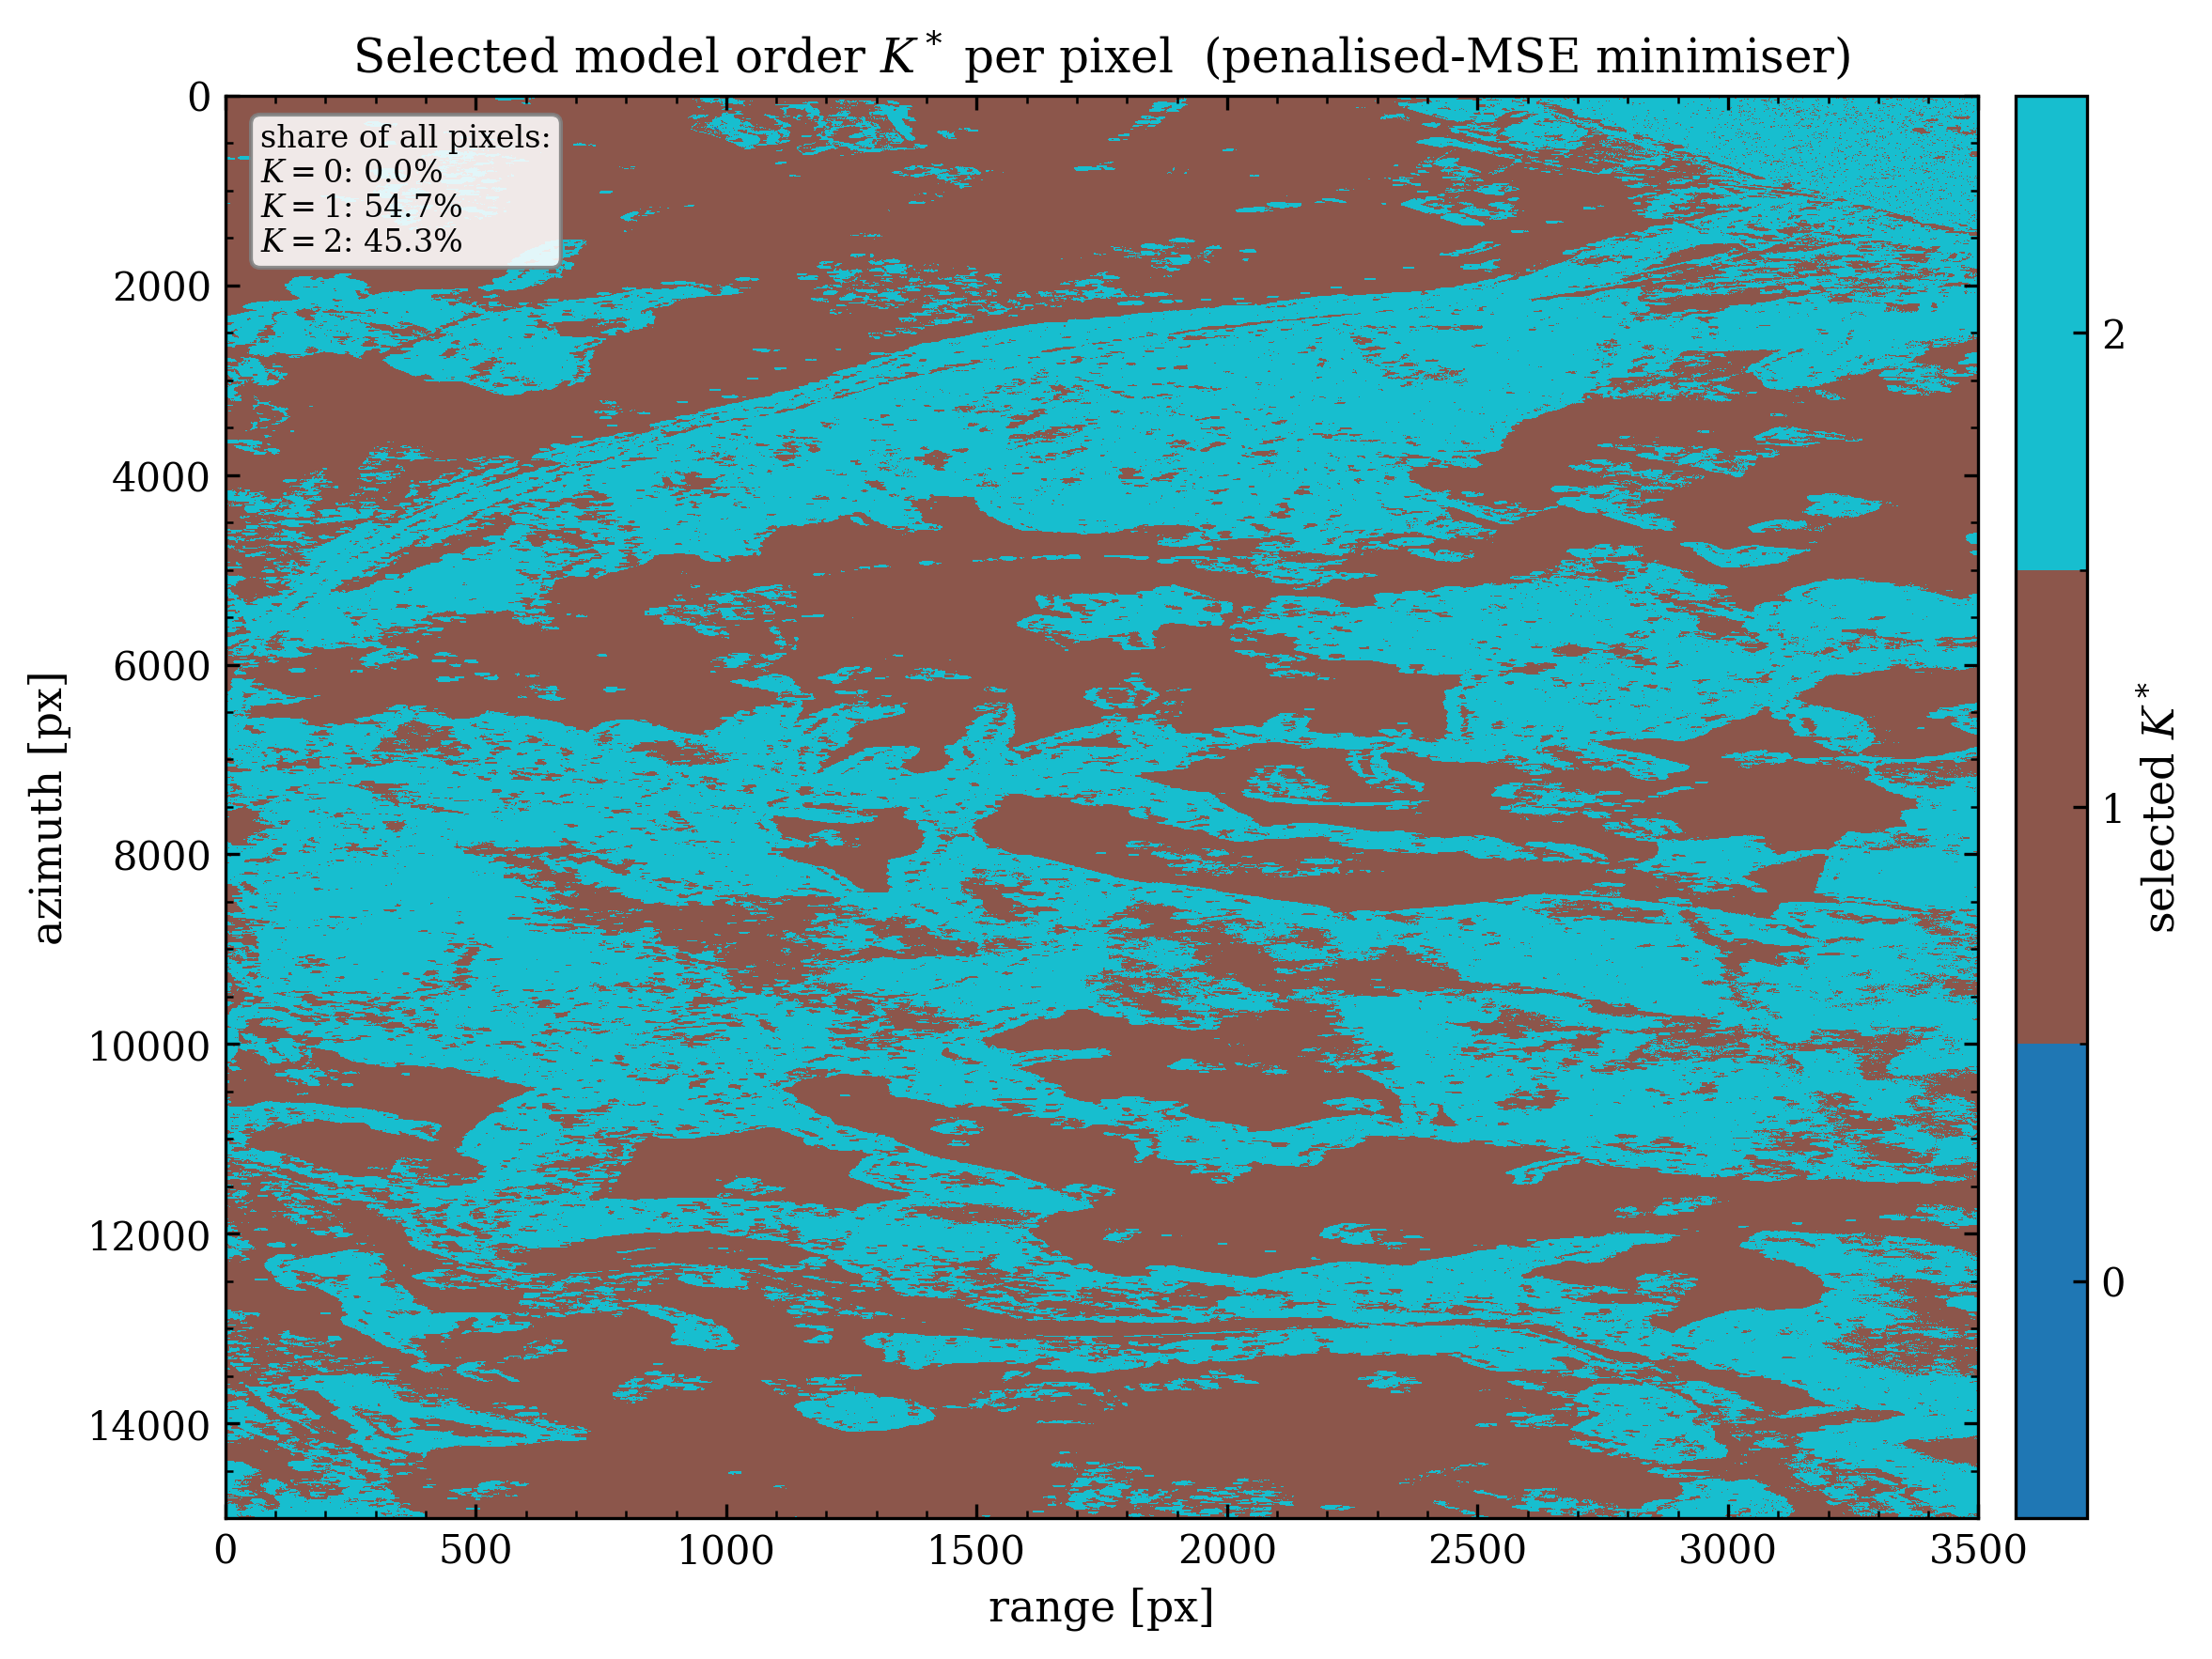
\includegraphics[width=\linewidth,height=0.8\textheight,keepaspectratio]{../figures/param_extraction/best_k_map.png}
    \end{column}
    \begin{column}{0.36\textwidth}
      \small
      \begin{itemize}
        \item The penalised-MSE selection of the previous slide, run per pixel over the full scene.
        \item \textbf{$K{=}1$: 54.7\%}, \textbf{$K{=}2$: 45.3\%}, $K{=}0$: 0.0\% --- the ``most pixels activate one or two Gaussians'' claim, now measured.
        \item The two orders track \textbf{spatial structure}: contiguous regions of single- vs double-scatterer response, following the scene's layover geometry --- not per-pixel noise.
        \item Rides with the dataset as a diagnostic; the complexity price $\lambda_K$ becomes load-bearing for the $K{=}5$ extension.
      \end{itemize}
    \end{column}
  \end{columns}
\end{frame}

% ---------------------------------------------------------------- 9 GT at scale
\begin{frame}{Label generation at scale: multi-GPU parameter extraction}
  \begin{columns}[c]
    \begin{column}{0.40\textwidth}
      \small
      \begin{itemize}\setlength{\itemsep}{10pt}
        \item The fit reformulated as batched gradient optimisation: vectorised over all
              pixels, sharded across GPUs --- full-scene extraction in $\sim$4 minutes.
        \item Labels stop being precious: sweeps over $K$, regularisation and fit modes are
              routine; datasets are regenerated, never patched.
      \end{itemize}
    \end{column}
    \begin{column}{0.58\textwidth}
      \centering
      \begin{tikzpicture}
        \node[gate,  text width=20mm] (tomo) at (0,5.4) {full Capon tomogram\\{\tiny one spectrum per pixel}};
        \node[box,   text width=32mm, anchor=north] (gpu) at (-2.0,3.08) {multi-GPU JAX framework\\{\tiny batched Adam, all pixels at once}\\{\tiny 4$\times$ NVIDIA A100 40\,GB}\\{\tiny 6912 CUDA cores each}\\{\tiny \textbf{$\sim$4 min per scene}}};
        \node[box, draw=argA!70, fill=argA!6, text width=30mm, anchor=north] (cpu) at (2.0,3.08) {CPU curve-fit library\\per-pixel loop, sequential\\{\tiny up to 120 cores}\\{\tiny \textbf{hours per scene}}};
        \node[box, draw=good!60, fill=good!7, text width=26mm] (lab) at (0,0.55) {fitted parameter labels\\{\tiny $(a_k,\mu_k,\sigma_k)$, $K$ Gaussians per pixel}\\{\tiny \textcolor{soft}{same classical fit, either route}}};

        \begin{scope}[shift={(-2.0,3.9)}]
          \foreach \i/\x in {0/-1.23,1/-0.41,2/0.41,3/1.23} {
            \draw[accent!70,thin,fill=accent!8,rounded corners=1pt] (\x-0.36,-0.135) rectangle (\x+0.36,0.135);
            \node[font=\tiny,text=accent] at (\x,0) {GPU \i};
          }
          \draw[accent!80,thick] (-1.23,0.45)  -- (1.23,0.45);
          \draw[accent!80,thick] (-1.23,-0.45) -- (1.23,-0.45);
          \foreach \x in {-1.23,-0.41,0.41,1.23} {
            \draw[accent!80,thin] (\x,0.45)  -- (\x,0.14);
            \draw[accent!80,thin] (\x,-0.14) -- (\x,-0.45);
          }
        \end{scope}
        \node[font=\tiny,text=accent!80,anchor=east] at (-2.13,3.27) {all pixels per step};

        \begin{scope}[shift={(2.0,3.9)}]
          \foreach \p in {-0.18,-0.06,0.06,0.18} {
            \draw[argA!80,thin] (\p,0.30)  -- (\p,0.39);
            \draw[argA!80,thin] (\p,-0.30) -- (\p,-0.39);
            \draw[argA!80,thin] (0.30,\p)  -- (0.39,\p);
            \draw[argA!80,thin] (-0.30,\p) -- (-0.39,\p);
          }
          \draw[argA!80,thick,fill=argA!5,rounded corners=1pt] (-0.30,-0.30) rectangle (0.30,0.30);
          \draw[argA!80,thin] (-0.19,-0.19) rectangle (0.19,0.19);
          \node[font=\tiny,text=argA] at (0,0) {CPU};
        \end{scope}
        \node[font=\tiny,text=argA!80,align=center,anchor=west] at (2.52,3.9) {one pixel\\per fit};

        \begin{scope}[on background layer]
          \fill[accent!5,rounded corners=3pt] (-3.85,0.0) rectangle (-0.06,5.85);
          \fill[argA!6,rounded corners=3pt]   (0.06,0.0)  rectangle (3.85,5.85);
          \draw[soft!50,dotted,very thick] (0,-0.15) -- (0,6.0);
        \end{scope}
        \node[font=\scriptsize\itshape,text=accent!80,anchor=south] at (-1.95,5.95) {fast axis};
        \node[font=\scriptsize\itshape,text=argA!80,anchor=south]   at (1.95,5.95)  {slow axis};

        \draw[accent!80,thick] (tomo.west) -| (-2.0,4.35);
        \draw[flow] (-2.0,3.45) -- (gpu.north);
        \draw[flow] (gpu.south) |- (lab.west);
        \draw[argA!80,thick] (tomo.east) -| (2.0,4.35);
        \draw[flow, argA!80] (2.0,3.45) -- (cpu.north);
        \draw[flow, argA!80] (cpu.south) |- (lab.east);
      \end{tikzpicture}
    \end{column}
  \end{columns}
\end{frame}
